\documentclass[french]{beamer}
\usepackage[utf8]{inputenc}
\usepackage[T1]{fontenc}
\usepackage{graphicx}

%\usepackage[abs]{overpic}
\graphicspath{{figures/}}
\usepackage{xcolor}
%\usetheme{Warsaw}

%%%%autre theme possible
\usetheme{Hannover}
\useoutertheme{infolines}
%%%%%%%%
\hypersetup{pdfpagemode=FullScreen}

\usepackage{siunitx}

\usepackage{caption}
\captionsetup{font=scriptsize,labelfont=scriptsize}
\setbeamertemplate{caption}[numbered]





\begin{document}

% \begin{frame}
%    \frametitle{Courbe en S}
%    \framesubtitle{Sommaire}
%    \tableofcontents[currentsection]
% \end{frame}

\AtBeginSection[]
{
  \begin{frame}
    \frametitle{Sommaire}
    \tableofcontents[currentsection]
  \end{frame}
}



%_______________________________________
\section{Présentation du problème}
\begin{frame}
\frametitle{Mise en équation}

   \begin{itemize}
      \item Équation thermique
      \begin{equation}
         Cv\frac{\partial T}{\partial t} = Q^+ + Q^- +Q^{adv}
      \end{equation}
      
   \item Équilibre thermique local
   \begin{equation}
      Q^+ = Q^- 
   \end{equation}
   
      \begin{itemize}
         \item état stationnaire
         \\
         \item dépend de la position
         \item courbes en S pour 256 valeurs du rayon
      \end{itemize}
\end{itemize}
\end{frame}
%_______________________________________

%_______________________________________
\section{Résolution des équations}
\begin{frame}
\frametitle{Résolution des équations}

   \begin{itemize}
      \item Ordre des équations
      \item Détermination de la température
      \item Méthodes de résolution
         \begin{itemize} 
            \item Dichotomie
            \item Amélioration de la dichotomie
            \item Méthode de Brent
            \item Comparaison des différentes méthodes
         \end{itemize}
      \item Épaisseur optique
   \end{itemize}
\end{frame}
%_______________________________________

%_______________________________________

%_______________________________________
%SCHEMA DU DISQUE
\begin{frame}
\frametitle{Ordre des équations}

   \begin{figure}[htb!]
      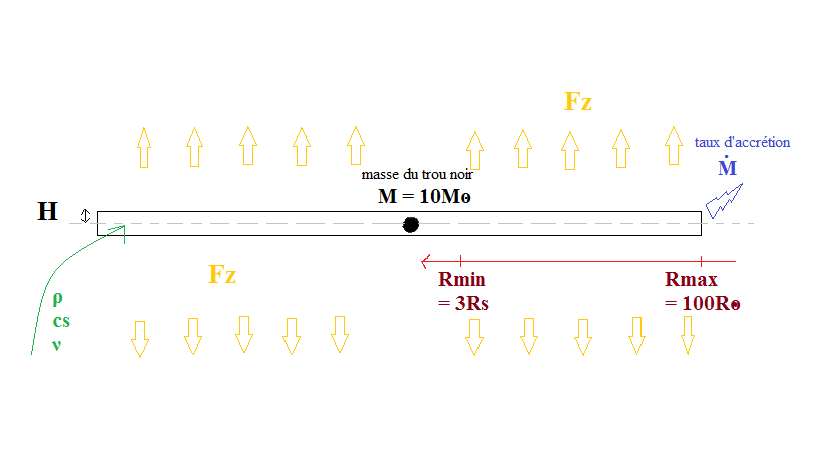
\includegraphics[width=7cm]{figures/bob_ross.png}
      \caption{Schéma très simplifié du disque d'accrétion autour d'un trou noir.}
   \end{figure}

   \begin{itemize}
      \item Demi-hauteur H du disque

      Solution d'une équation quadratique trouvée à partir de la pression :
      \begin{equation}
         P = P_\mathrm{gaz} + P_\mathrm{rad}
      \end{equation}
      
      \item Densité volumique $\rho$
      \item Vitesse du son $c_s$ 
      \item Viscosité $\nu$ 
      \item Flux radiatif $F_z$
      
      2 approximations en fonction de la profondeur optique $\tau_{eff}$
   \end{itemize}
\end{frame}
%_______________________________________


%_______________________________________

\begin{frame}
\frametitle{Détermination de l'intervalle de Température} 

   \begin{equation}
      L_\mathrm{Edd} = \frac{4\pi GMm_pc}{\sigma_e}
   \end{equation}

   puis celle permettant de définir le taux d’accrétion critique 
   \begin{equation}
      \dot{M}_\mathrm{crit} = \frac{12}{c^2}L_\mathrm{Edd} 
   \end{equation}

   ce qui nous donne une valeur de la température caractéristique $T_0$
   \begin{equation}
      T_0 \approx 2,50.10^7\left(\frac{\dot{M}_0}{\dot{L}_\mathrm{crit}}\right)^{\frac{1}{4}}\left(\frac{M}{M_\odot}\right)^{-\frac{1}{4}} \mathrm{K}
   \end{equation}


\end{frame}
%_______________________________________


%_______________________________________

\begin{frame}
\frametitle{Détermination de l'intervalle de Température} 

   Finalement : 
\begin{eqnarray}


   T_0 =1.40\ 10^6 \mathrm{K} 
   
   T_\textrm{min} = 2.9\ 10^5 \mathrm{K}
    
   T_\textrm{max} = 6.2\ 10^6 \mathrm{K} 
\end{eqnarray}

\end{frame}
%_______________________________________


%_______________________________________

\begin{frame}
\frametitle{Dichotomie}

   \begin{itemize}
      \item Racine $f(\Sigma) = Q^+ - Q^- = 0$ comprise dans un intervalle $[\Sigma_{min}$ ; $\Sigma_{max}]$
      \\
      \begin{figure}[htb!]
         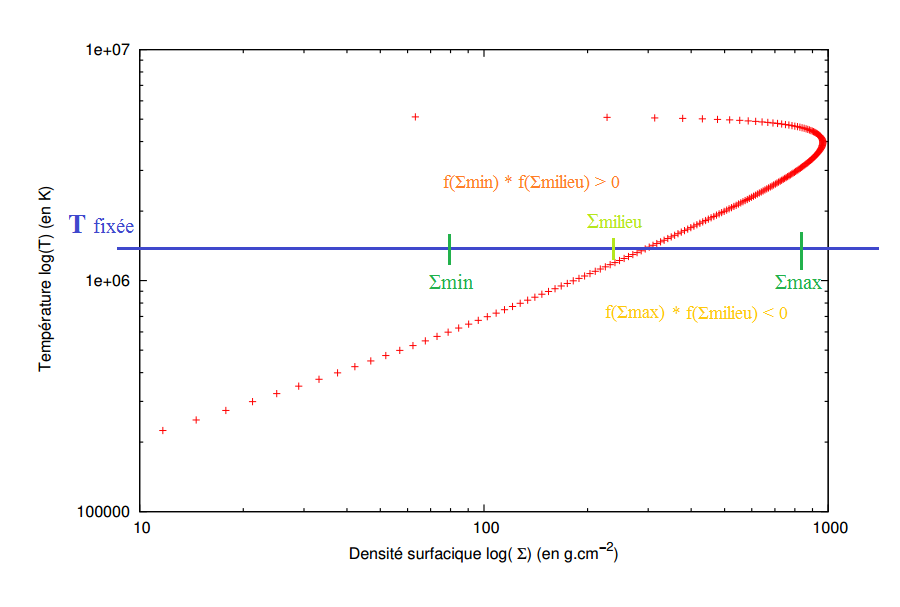
\includegraphics[width=8cm]{figures/dicho_1.png}
      \end{figure}
   \end{itemize}
\end{frame}
%_______________________________________

%_______________________________________

\begin{frame}
\frametitle{Dichotomie}

   \begin{itemize}
      \item Racine $f(\Sigma) = Q^+ - Q^- = 0$ 
      
      comprise dans un intervalle $[\Sigma_{min}$ ; $\Sigma_{max}]$
      \\
      \begin{figure}[htb!]
         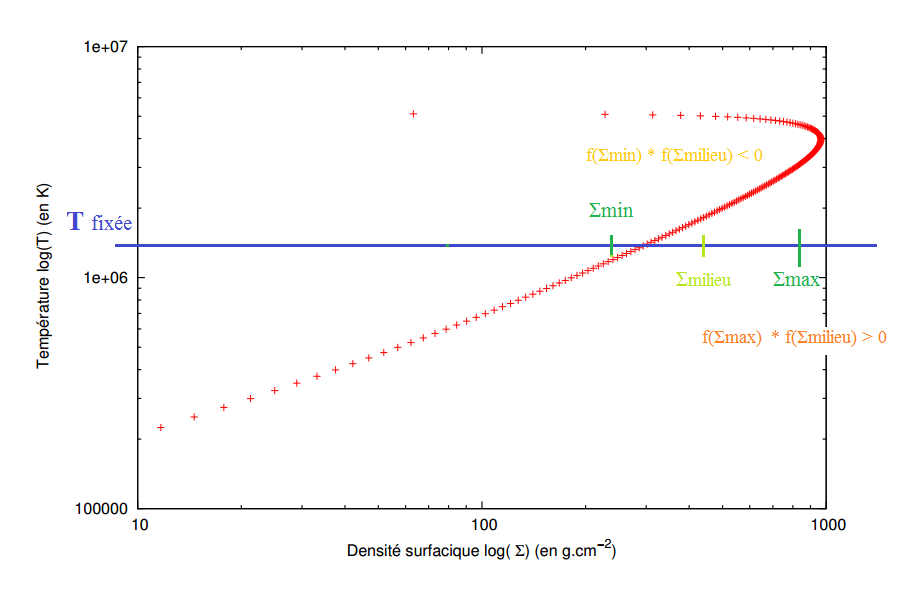
\includegraphics[width=8cm]{figures/dicho_2.png}
      \end{figure}
   \end{itemize}
\end{frame}
%_______________________________________


%_______________________________________

\begin{frame}
\frametitle{Amélioration de la dichotomie}
\framesubtitle{Méthode de Newton}
%\setbeamertemplate{itemize item}[square]

   \begin{itemize}
      \item Présentation
      \\
      \begin{equation}
         x_{k+1} = x_k - \frac{f(x_k)}{f'(x_k)}
      \end{equation}

      \begin{figure}[htb!]
         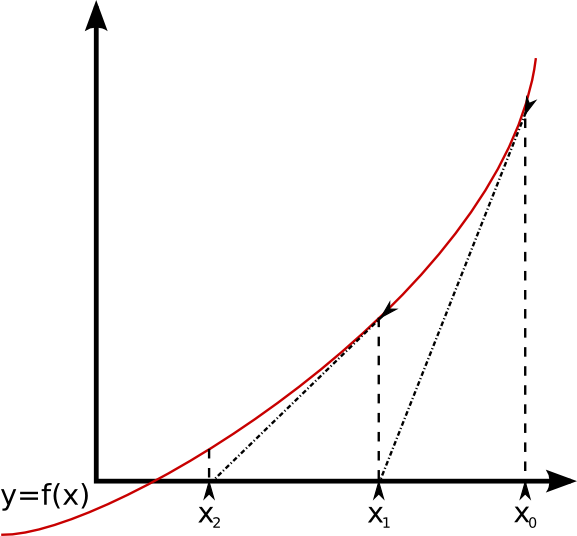
\includegraphics[width=3cm]{figures/Newton_method.png}
         \caption{Illustration de la méthode de Newton. Crédit: Wikimedia Commons}
      \end{figure}

   \end{itemize}
\end{frame}
%_______________________________________

%_______________________________________

\begin{frame}
\frametitle{Amélioration de la dichotomie}
\framesubtitle{Méthode de Newton}
%\setbeamertemplate{itemize item}[square]

   \begin{itemize}
      \item Avantages :
         \begin{itemize}
            \item Convergence quadratique
         \end{itemize}
      \item Inconvénients :
      \begin{itemize}
         \item Nécessite le calcul littéral de la dérivée.
         \item La fonction doit être obligatoirement de classe $C^1$.
         \item S'il existe plusieurs racines, ne converge pas forcément vers la plus proche du point de départ.
      \end{itemize}
   \end{itemize}
\end{frame}
%_______________________________________

%_______________________________________

\begin{frame}
\frametitle{Méthode de Brent}

Combinaison des méthodes de la dichotomie, de la sécante et l'interpolation quadratique inverse pour en utiliser tous leurs avantages.

   \begin{itemize}
      \item Méthode quadratique inverse

      \begin{equation}
         s = \frac{af(b)f(c)}{(f(a)-f(b))(f(a)-f(c))} 
  + \frac{\textsl{•}bf(a)f(c)}{(f(b)-f(a))(f(b)-f(c))}
  + \frac{cf(a)f(b)}{(f(c)-f(a))(f(c)-f(b))}
     \end{equation}

     \item Méthode de la sécante

     \begin{equation}
        x_{n+1} = x_n - \frac{x_n - x_{n-1}}{f(x_n) - f(x_{n-1})}
     \end{equation}

   \end{itemize}
\end{frame}
%_______________________________________


%_______________________________________

\begin{frame}
\frametitle{Méthode de Brent}

   \begin{itemize}
      \item Si le dénominateur ne s'annule pas, on utilise la méthode quadratique inverse.
      \item Autrement on utilise la méthode de la sécante sauf s'il on est trop éloigné de la solution.
      \item Dans ce cas, on utilise la méthode de la dichotomie.
   \end{itemize}
\end{frame}
%_______________________________________


%_______________________________________

\begin{frame}
\frametitle{Comparaison des différentes méthodes}

   \begin{figure}[htb!]
      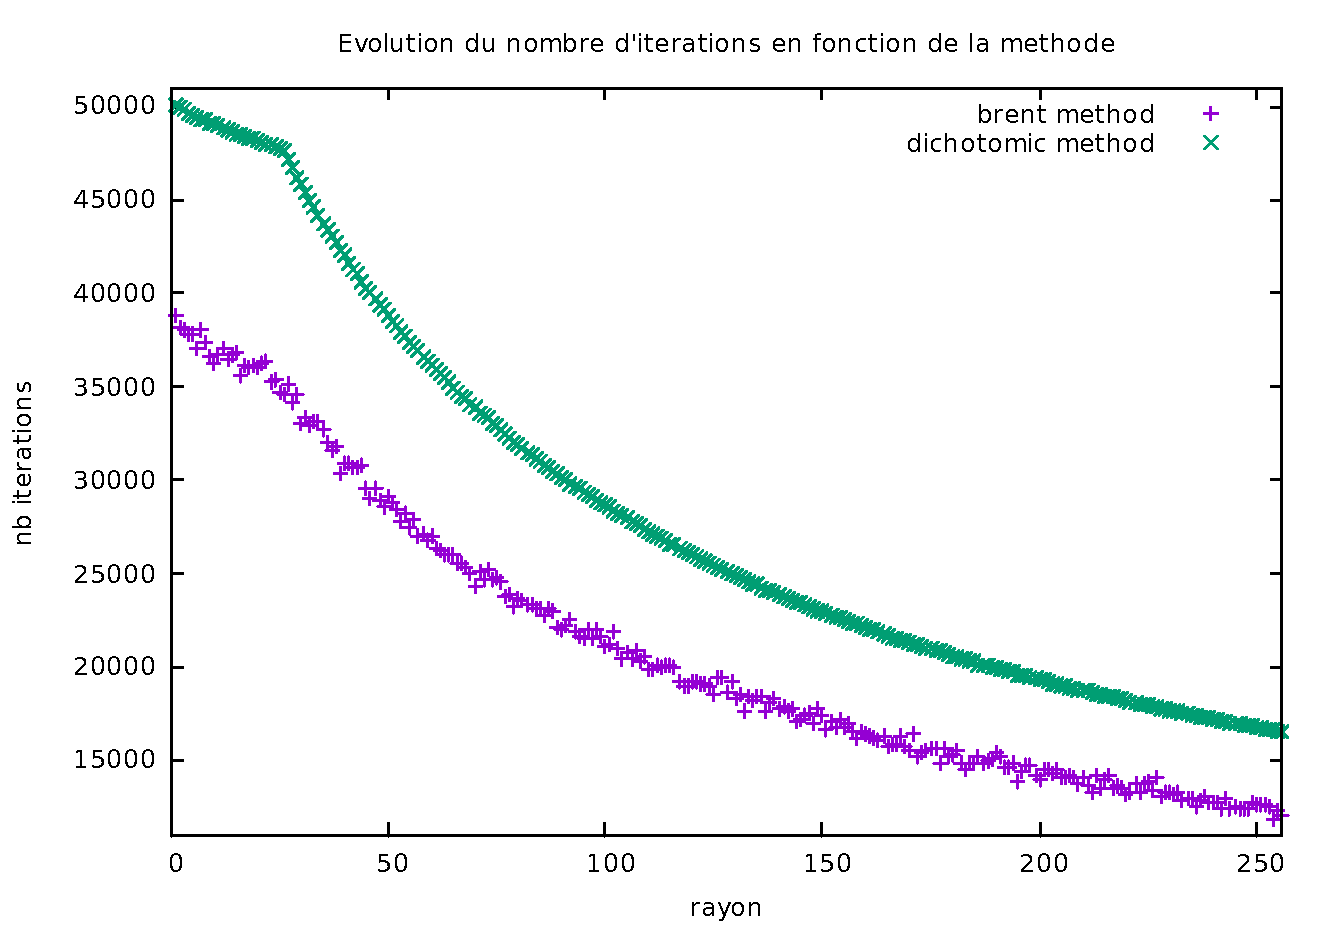
\includegraphics[width=9cm]{figures/brent_method3.pdf}
   \end{figure}
\end{frame}
%_______________________________________

%_______________________________________

\begin{frame}
\frametitle{Comparaison des différentes méthodes}

   \begin{tabular}{|c|c|c|}
     \hline
        Méthode & + & - \\
     \hline
     \\
     Dichotomie & simple & beaucoup d'itérations  
     \\  
     \hline
     \\
     Newton & plus rapide  & fonction dérivable 
     \\ 
     \hline
     \\  
     Sécante & pas de dérivée & intervalle de départ 
     \\  
     \hline  
     \\  
     Brent & interpolation quadratique inverse & convergence rapide 
     \\  
     \hline
   \end{tabular}
\end{frame}
%_______________________________________


%_______________________________________

\section{Détermination des points critiques}
\begin{frame}
\frametitle{Zones de stabilité}

   \begin{figure}[htb!]
      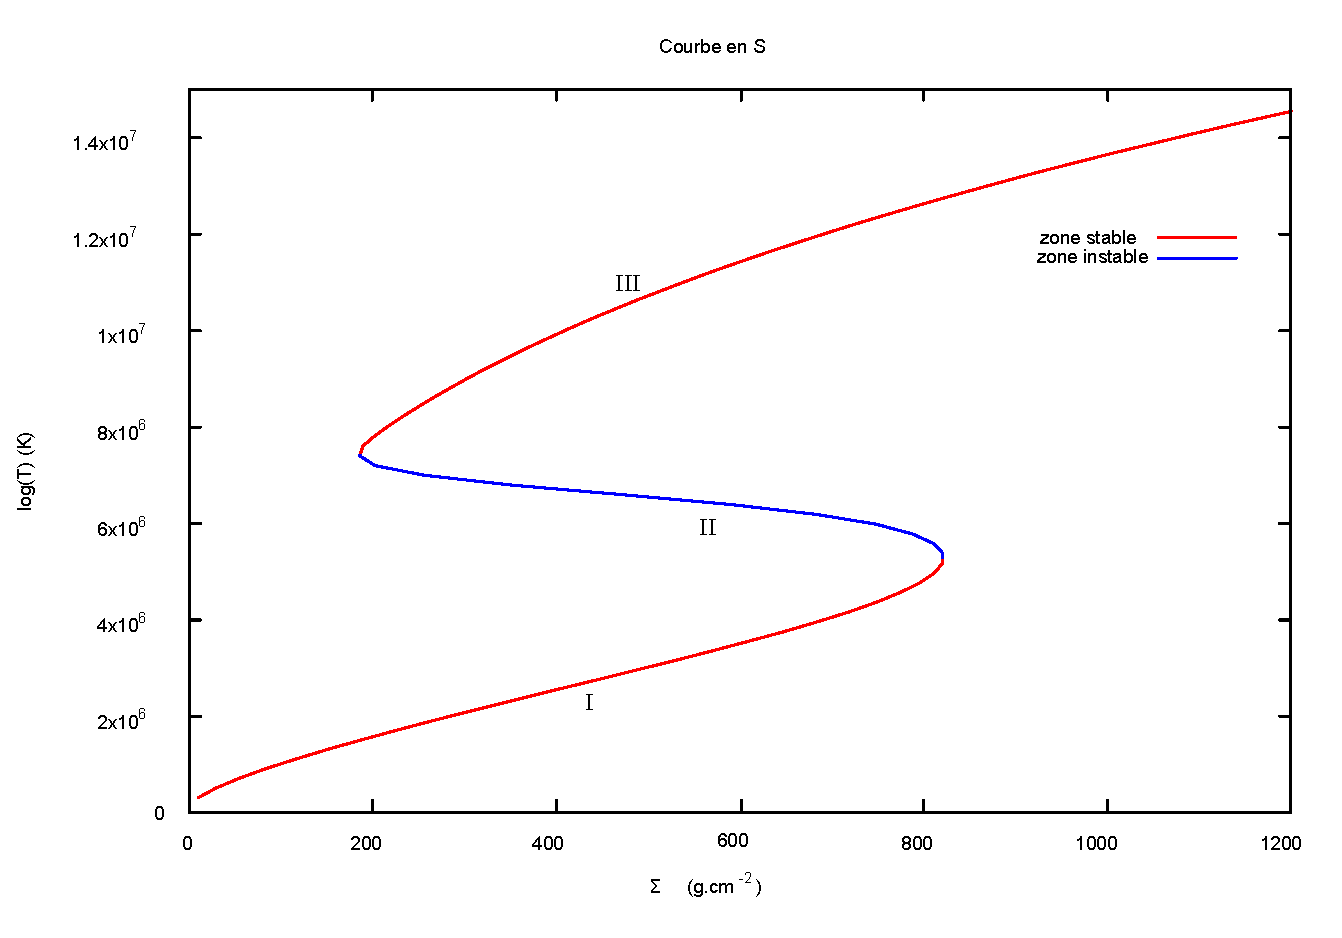
\includegraphics[width=8cm]{figures/stable.pdf}
      %LOG!!!
      \caption{Zones de stabilités de la courbe en S.}
    \end{figure}
\end{frame}
%_______________________________________

\begin{frame}		
\frametitle{Points critiques}		
		
   \begin{figure}[htb!]		
      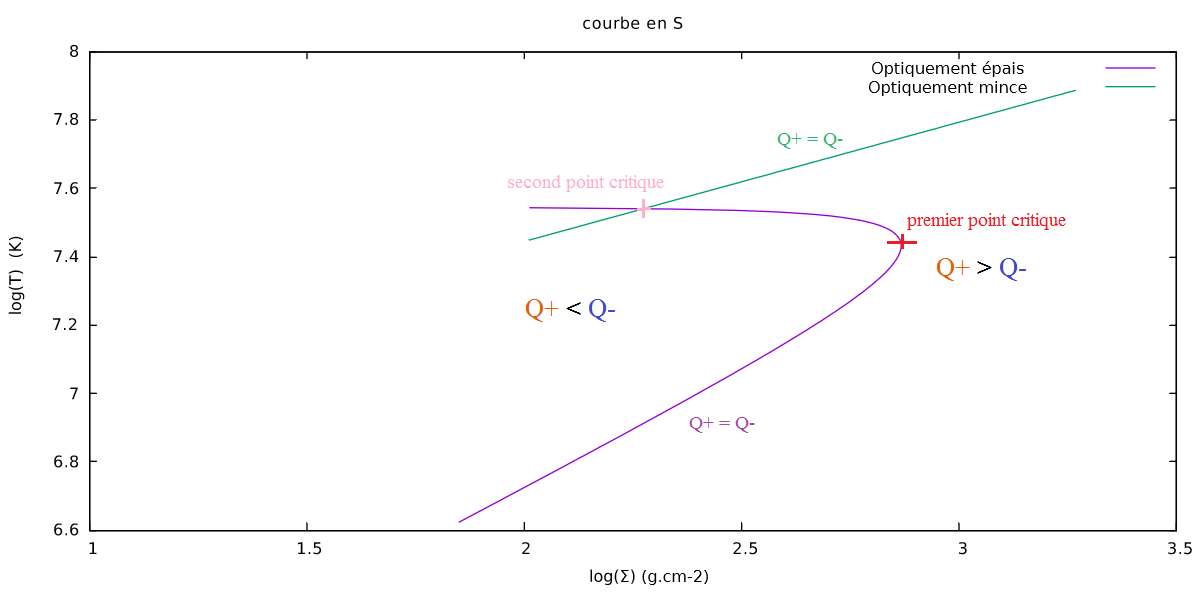
\includegraphics[width=8cm]{figures/points_critiques.png}		
      \caption{Localisation des points critiques sur la courbe en S.}		
    \end{figure}		
\end{frame}		


%_______________________________________

\section{Épaisseur optique}
\begin{frame}

   \begin{figure}[htb!]
      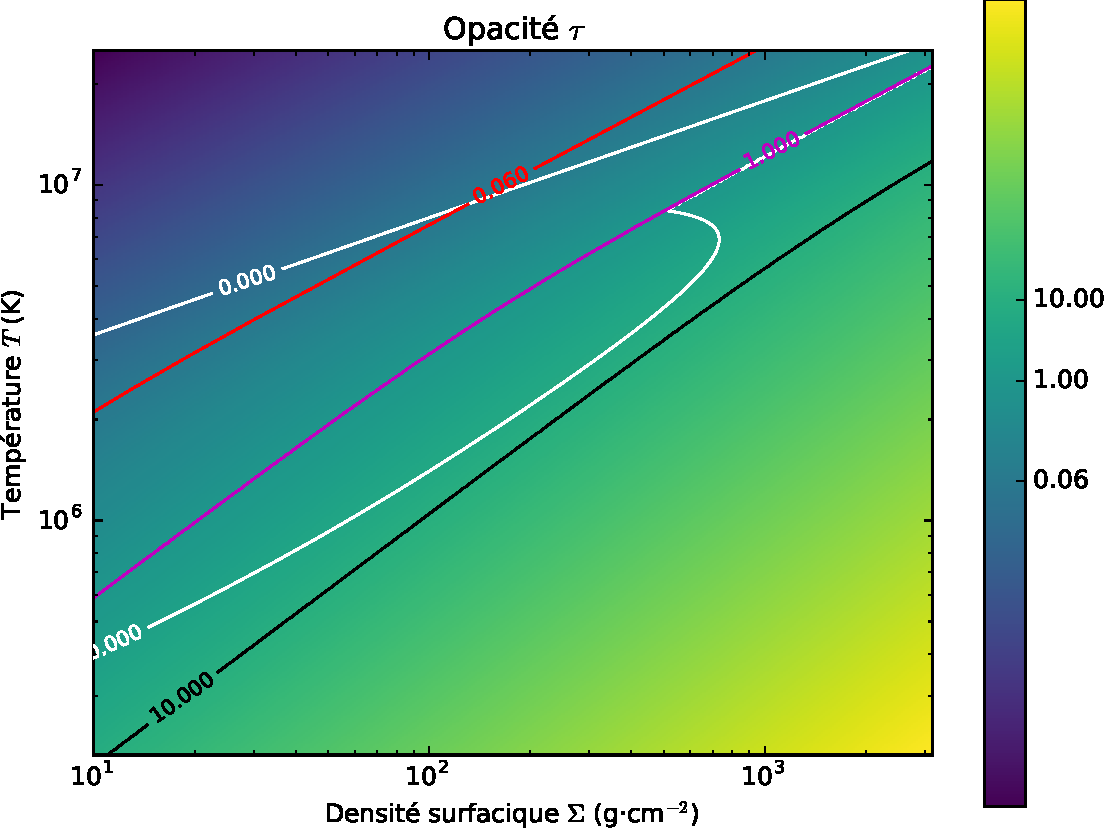
\includegraphics[width=8cm]{figures/tau_map.pdf}
      %\caption{ }
   \end{figure}
\end{frame}
%_______________________________________

%_______________________________________
\section{Différence des termes Q+ et Q-}
\begin{frame}

   \begin{figure}[htb!]
      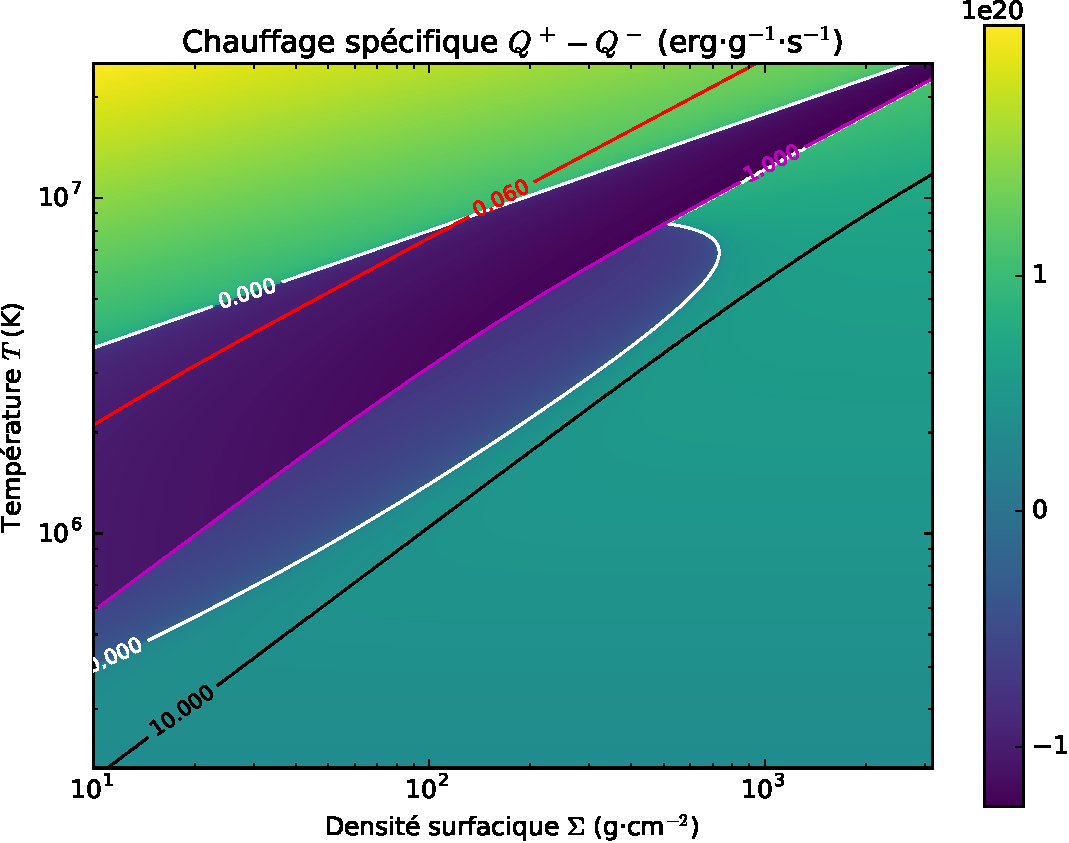
\includegraphics[width=8cm]{figures/Qmap.pdf}
     %\caption{ }
   \end{figure}
\end{frame}
%_______________________________________

%_______________________________________

\section{Discussion et conclusion}
\begin{frame}

   \begin{itemize}
      \item Non unicité des racines de $f(\Sigma) = 0$
      \\
         \begin{itemize}
            \item Interpolation du $\tau_{eff} \approx 1$ critique
            \item Existance de plusieurs branches minces ? 
         \end{itemize}  
      \item $\tau_{eff} \simeq 0.06 et \neq 1$ 
      \\
Simulation en accord avec la valeur théorique
   \end{itemize}
\end{frame}
%_______________________________________

%_______________________________________

\begin{frame}

   \begin{figure}[htb!]
      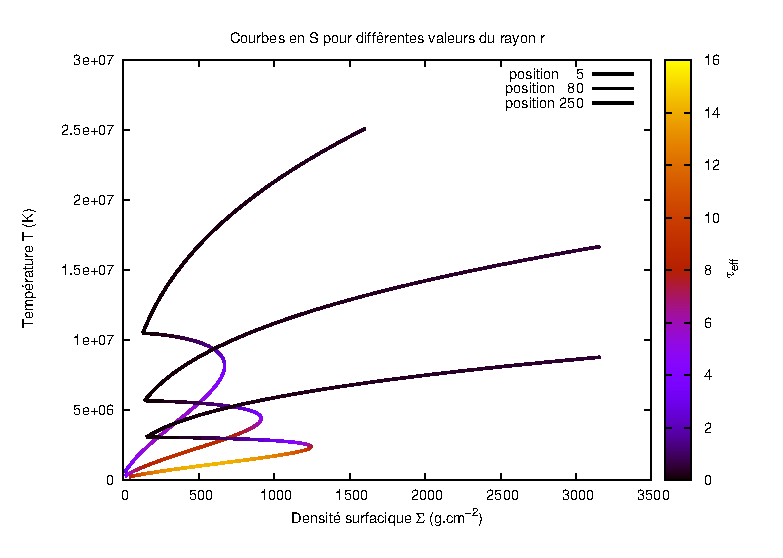
\includegraphics[width=9cm]{figures/S_curves_tau.eps}
      %\caption{ }
   \end{figure}
\end{frame}
%_______________________________________
%Parie équations adimmensinnement, CI et modèle alpha
\section{Les variables du modèle}
\begin{frame}
\begin{itemize}
	\item 6 paramètres d'entrée :
	\begin{itemize}
		\item $M$ : masse du trou noir
		\item $r_{max}$ = rayon maximal du trou noir
		\item $X$ : fraction en masse d'hydrogène
		\item $Y$ : fraction en masse d'hélium
		\item $\dot{M}_{0}$ : taux d'accrétion au bord du disque
		\item $\alpha$ : paramètre phénoménologique libre 
	\end{itemize}
\end{itemize}
\end{frame}

\begin{frame}
\begin{itemize}
	\item {Tableau récapitulatif des variables}
\end{itemize}

\begin{center}
    \begin{tabular}{|c|c|c|}
        \hline
        Variable & Variable adimensionnée & Adimensionnement \\
        \hline
        $\Omega$ & $\Omega^\star = \Omega/\Omega_0$ & $\Omega_0 = \left( \frac{G M}{r^3_s} \right)^\frac{1}{2}$ \\
        $t$ & $t^\star = t/t_0$ & $t_0 = 2 \Omega_0^{-1}$ \\
        $r$ & $x = \sqrt{r/r_s}$ & N/A \\
        $\nu$ & $\nu^\star = \nu/\nu_0$ & $\nu_0 = \frac{4 r_s^2}{3 t_0} = \frac{2 r_s^2 \Omega_0}{3}$ \\
        $v$ & $v^\star = v/v_0$ & $v_0 = 2 \frac{r_s}{t_0} = r_s \Omega_0$ \\
        $c_s$ & $c_s^\star = c_s/c_s^0$ & $c_s^0 = v_0$ \\
        $\Sigma$ & $\Sigma^\star = \Sigma/\Sigma_0$ & $\Sigma_0 = \frac{\dot{M_0}}{3 \pi \nu_0}$ \\
        $S = \Sigma x$ & $S^\star = S/S_0 = \Sigma^\star x$ & $S_0 = \Sigma_0$ \\
        \hline
    \end{tabular}
\end{center}

\end{frame}

\begin{frame}
\begin{center}
    \begin{tabular}{|c|c|c|}
        \hline
        Variable & Variable adimensionnée & Adimensionnement \\
        \hline
         $H$ & $H^\star = H/H_0$ & $H_0 = r_s$ \\
        $\dot{M}$ & $\dot{M^\star} = \dot{M}/\dot{M_0}$ & N/A \\
        $\rho$ & $\rho^\star = \rho/\rho_0$ & $\rho_0 = \frac{\Sigma_0}{2 H_0} = \frac{\Sigma_0}{2 r_s}$ \\	
        $T$ & $T^\star = T/T_0$ & $T_0 = \left(\frac{1}{\sqrt{27}} \times \frac{\dot{M_0} c^2}{48 \pi r_s^2 \sigma} \right)^\frac{1}{4}$ \\
$F_z$ & $F_z^\star = F_z/F_z^0$ & $F_z^0 = \frac{\Sigma_0}{2 t_0} = \frac{\rho_0 H_0}{t_0} = \frac{\Sigma_0 \Omega_0}{4}$ \\
        $C_v$ & $C_v^\star = C_v/C_v^0$ & $C_v^0 = T_0^{-1}$ \\
        $P_\mathrm{gaz}$ & $P_\mathrm{gaz}^\star = P_\mathrm{gaz}/P_\mathrm{gaz}^0$ & $P_\mathrm{gaz}^0 = \frac{\rho_0 k_B T_0}{\mu m_p}$ \\
        $P_\mathrm{rad}$ & $P_\mathrm{rad}^\star = P_\mathrm{rad}/P_\mathrm{rad}^0$ & $P_\mathrm{rad}^0 = \frac{1}{3} a T_0^4$ \\
	     \hline
    \end{tabular}
\end{center}
\end{frame}

\begin{frame}
	\begin{subequations}
    \begin{align}
        \frac{\partial S^\star}{\partial t^\star} &= \frac{1}{x^2} \frac{\partial^2}{\partial x^2} \left(\nu^\star S^\star\right) \\
        v^\star &= - \frac{1}{S^\star x} \frac{\partial}{\partial x} \left(\nu^\star S^\star\right) \\
        \nu^\star &= \alpha c_s^\star H^\star \\
        c_s^\star &= \Omega^\star H^\star \\
        \Sigma^\star &= \frac{S^\star}{x} \\
        \dot{M^\star} &= - x S^\star v^\star \\
        \rho^\star &= \frac{S^\star}{x H^\star} \\
    \end{align}
\end{subequations}
\end{frame} 



\begin{frame}
	\begin{subequations}
    \begin{align}
    C_v^\star \frac{\partial T^{\star}}{\partial t^{\star}} &=
        3 v_0^2 \nu^\star {\Omega^\star}^2 - \frac{F_z^\star x}{S^\star} +
        \frac{\mathcal{R} T_0}{\mu} \frac{4-3\beta}{\beta} \frac{T^\star}{S^\star} \times
        \left( \frac{\partial S^\star}{\partial t^\star} + v^\star \frac{\partial}{\partial x} \left(\frac{S^\star}{x}\right) \right) -
        \frac{C_v^\star v^\star}{x} \frac{\partial T^\star}{\partial x}\\
        F_z^\star &=
        \begin{cases}
            \frac{2 c^2 x {T^\star}^4}{27 \sqrt{3} (\kappa_\mathrm{ff} + \kappa_e) S^\star \Sigma_0}, &\text{si $\tau_\mathrm{eff} \geq 1$} \\
            \frac{t_0}{\rho_0}\epsilon_\mathrm{ff} H^\star, &\text{si $\tau_\mathrm{eff} < 1$}
        \end{cases} \\
        \kappa_\mathrm{ff} &= \num{6.13e22} (\rho_0 \rho^\star) {T_0 T^\star}^{-\frac{7}{2}} \si{\square\centi\meter\per\gram} \\
        \kappa_e &= 0.2 \times (1 + X) \si{\square\centi\meter\per\gram} \approx \SI{0.34}{\square\centi\meter\per\gram} \\
        \epsilon_\mathrm{ff} &= \num{6.22e20} \times \rho^2 T^\frac{1}{2} \mathrm{cgs} \\
        \tau_\mathrm{eff} &= \frac{1}{2} (\kappa_e \kappa_\mathrm{ff})^\frac{1}{2} \frac{S^\star}{x} \Sigma_0 \\
    \end{align}
\end{subequations}
\end{frame} 

\begin{frame}
	\begin{subequations}
    \begin{align}
     C_v^\star &= \frac{\mathcal{R} T_0}{\mu} \frac{12 (\gamma_g - 1)(1 - \beta) + \beta}{(\gamma_g - 1) \beta} \\
        P_\mathrm{gaz}^\star &= \rho^\star T^\star \\
        P_\mathrm{rad}^\star &= {T^\star}^4 \\
        \beta &= \frac{1}{1 + \beta_0 \frac{{T^\star}^3}{\rho^\star}} = \frac{P_\mathrm{gaz}^\star}{P_\mathrm{gaz}^\star + \beta_0 P_\mathrm{rad}^\star} ; \beta_0 = \frac{P_\mathrm{rad}^0}{P_\mathrm{gaz}^0}
    \end{align}
\end{subequations}

	\begin{itemize}
		\item Calcul de la demi-hauteur du disque $H$ : Résolution par trinôme
	\end{itemize}
	
\end{frame} 

	\section{Les conditions initiales}
\begin{frame}
	\begin{equation}
	\dot{M} = 1\ 10^{-1 }\dot{M_{0}}
\end{equation} 

\begin{equation}
	T = 1.4 \times 10^{4} \alpha^{- \frac{1}{5}} \left[ \frac{\dot{M}}{10^{16} \mathrm{g.s}^{-1}} \right]^{\frac{3}{10}} \left[ \frac{M}{M_\odot}\right]^{\frac{1}{4}} \left[ \frac{r}{10^{10}\mathrm{cm}}\right]^{- \frac{3}{4}} f^{\frac{3}{10}} \mathrm{K} 
\end{equation}

\begin{align}
	\Sigma = 5.2 \alpha^{- \frac{4}{5}} \left[ \frac{\dot{M}}{10^{16} \mathrm{g.s}^{-1}} \right]^{\frac{7}{10}} \left[ \frac{M}{M_\odot}\right]^{\frac{1}{4}} \left[ \frac{r}{10^{10} \mathrm{cm}}\right]^{- \frac{3}{4}} f^{\frac{7}{10}} \mbox{K}  \\ 
	\text{avec } f = \left[ 1 - \left( \frac{r}{3 r_{s}}\right)^{- \frac{1}{2}}\right]
\end{align}
\end{frame}

\begin{frame}
 \begin{figure}[ht]
   \begin{minipage}[c]{.46\linewidth}
      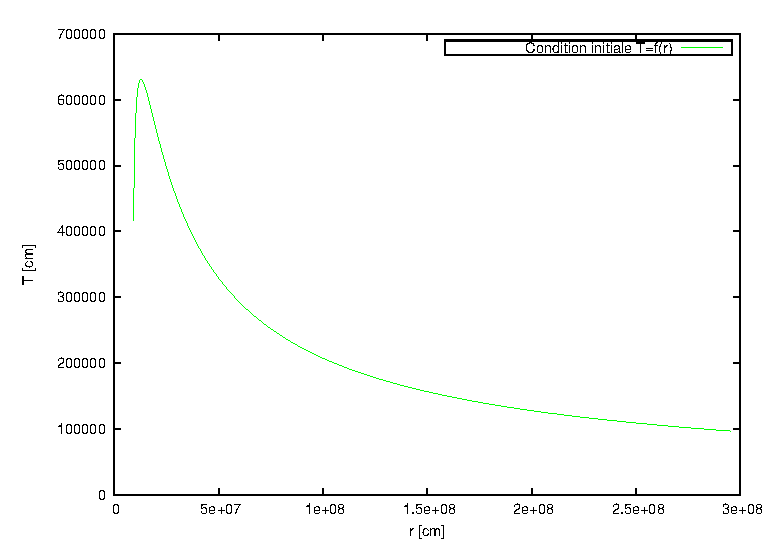
\includegraphics[scale=0.42]{ic_T.eps}
      \caption{Tracé de $T(r)$ à $t = 0$}
   \end{minipage} \hfill
   \begin{minipage}[c]{.46\linewidth}
      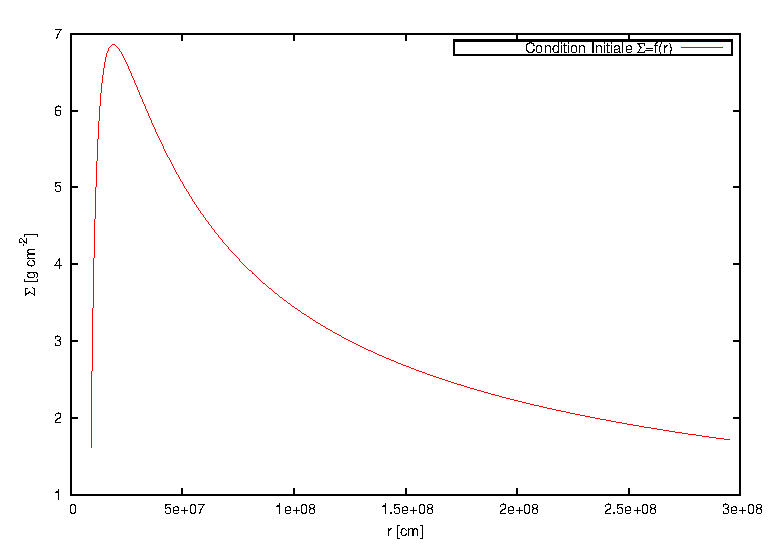
\includegraphics[scale=0.42]{ic_Sig.eps}
      \caption{Tracé de $\Sigma(r)$ à $t = 0$}
   \end{minipage}
\end{figure} 
\end{frame}

\begin{frame}
	\begin{equation}
	\frac{H}{r} = 1.7 \times 10^{-2}\alpha^{- \frac{1}{10}} \left[ \frac{\dot{M}}{10^{16} \mbox{g} \mbox{s}^{-1}} \right]^{\frac{3}{20}} \left[ \frac{M}{M_\odot}\right]^{- \frac{3}{8}} \left[ \frac{r}{10^{10} \mathrm{cm}}\right]^{- \frac{1}{8}} f^{\frac{3}{5}}
\end{equation}
\end{frame}

\begin{frame}
	\begin{center}
		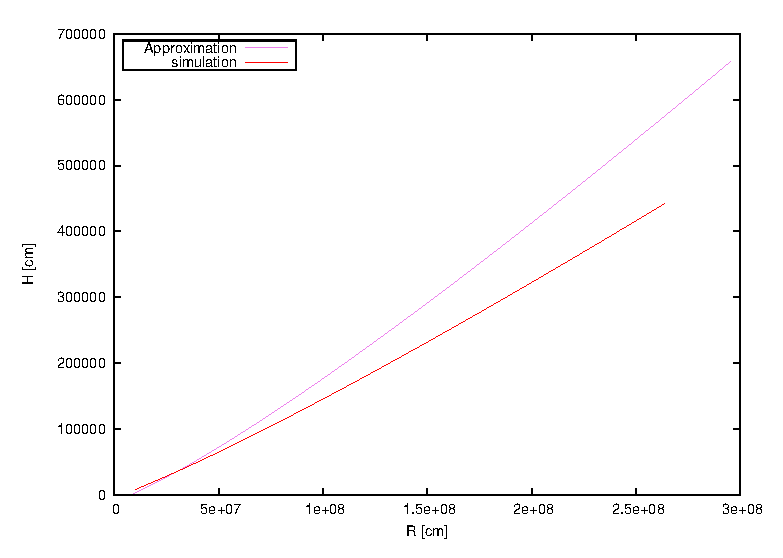
\includegraphics[scale=0.7]{ic_h.eps}
	\end{center}
\end{frame}

\begin{frame}
	\begin{center}
		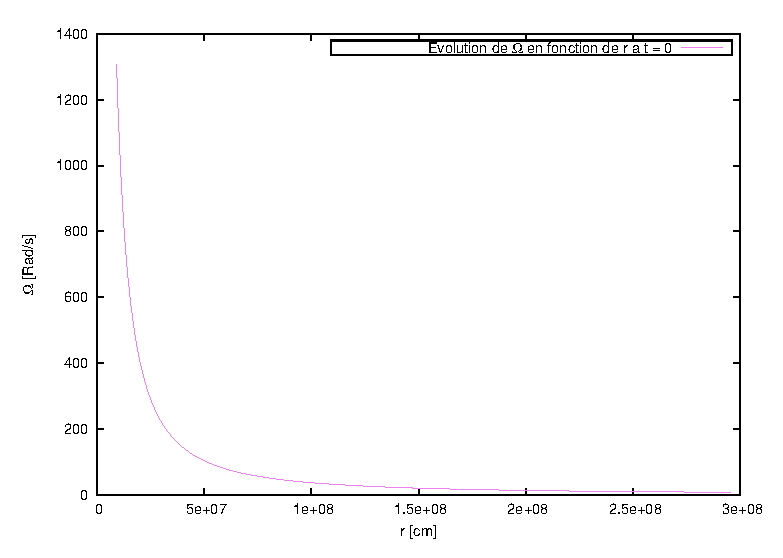
\includegraphics[scale=0.7]{Omega.eps}
	\end{center}
\end{frame}



%_______________________________________
\section{Intégration}

\section{Condition aux bords}


%---------------------------
\begin{frame}
\frametitle{Dérivation Spatiale}

On utilise la Dérivée dite \textit{amont} : 

\begin{equation*}
\left. \frac{\partial \nu^{\star} S^{\star}}{\partial x} \right|_i = \frac{\nu^{\star}S^{\star}(i+1)-\nu^{\star}S^{\star}(i)}{\delta x} 
\end{equation*}


Quand $i=i_{max} \rightarrow \nu^{\star}S^{\star}(i_{max}+1) $??

\end{frame}
%---------------------------


%---------------------------
\begin{frame}
\frametitle{Grandeur à dérivé}
Dérivées spatiale intervenant :

\begin{itemize}
    \item dérivé première
    \begin{itemize}
        \item $T^*$
        \item $ \nu^{\star}S^{\star}$
        \item $\frac{S^{\star}}{x}$
    \end{itemize}
    \item dérivée seconde :
    \begin{itemize}
        \item $ \nu^{\star}S^{\star}$
    \end{itemize}
\end{itemize}

\end{frame}
%---------------------------


%---------------------------
\begin{frame}
\frametitle{Conditions aux bords}
\framesubtitle{$T^*$ ; $\nu^{\star} S^{\star}$}

\begin{itemize}

\onslide<1->
\item $\left.\frac{\partial T^{\star}}{\partial x}\right|_{i_{max}} =0$ par condition sur notre modèle

\onslide<2->
\item $\dot{M}^{\star} = \frac{\partial \nu^{\star} S^{\star}}{\partial x}$ Donc $ (\dot{M_0}^{\star} =)1= \left. \frac{\partial \nu^{\star} S^{\star}}{\partial x} \right|_{i_{max}} $

\end{itemize}

\end{frame}
%---------------------------

%---------------------------
\begin{frame}
\frametitle{Condition aux bords}
\framesubtitle{$\nu^{\star} S^{\star}$}

\only<1-3>{
$$\left. \frac{\partial \nu^{\star} S^{\star}}{\partial x} \right|_{i_{max}} = 1 = \frac{\nu^{\star}S^{\star}(i_{max}+1)-\nu^{\star}S^{\star}(i_{max})}{\delta x} $$ 
}
\only<2-3>{
On en déduit 

$$\nu^{\star}S^{\star}(i_{max}+1) = \delta x + \nu^{\star}S^{\star}(i_{max})$$ 
}

\only<3>{
Donc 
$$  \left. \frac{\partial^2 (\nu^{\star} S^{\star})}{\partial x^2}\right|_{i=i_{max}} = \frac{\delta x - (\nu^{\star} S^{\star})(i_{max}) + (\nu^{\star} S^{\star})(i_{max}-1)}{\delta x^2}$$
}

\only<4>{
en $i=0$ on a  $ \nu^{\star} S^{\star} =0$  d'où 
$$ \left. \frac{\partial^2 \nu^{\star}S^{\star}}{\partial x^2}\right|_{i=1}=\frac{(\nu^{\star}S^{\star})(1+1)-2\ (\nu^{\star}S^{\star})(1)}{\delta x^2}$$
 }
\end{frame}
%---------------------------

%---------------------------
\begin{frame}
\frametitle{Conditions aux bords}
\framesubtitle{$S^*/x$}

En $i_{max}$ 
$$Q_{adv}=\frac{\mathcal{R} T_0}{\mu} \frac{4-3\beta}{\beta} \frac{T^\star}{S^\star} \times
        \left( \frac{\partial S^\star}{\partial t^\star} + v^\star \frac{\partial}{\partial x} \left(\frac{S^\star}{x}\right) \right) -
        \frac{C_v^\star v^\star}{x} \frac{\partial T^\star}{\partial x}=0 $$

Donc
$$  \frac{\partial}{\partial x} \left(\frac{S^{\star}}{x}\right) = - \frac{1}{v^{\star}} \frac{\partial S^{\star}}{\partial t^{\star}} $$

$$ \left. \frac{\partial}{\partial x} \left(\frac{S^{\star}}{x}\right) \right|_{i_{max}} = \left. -\frac{1}{x^2\ v^{\star}} \frac{\partial^2 (\nu^{\star} S^{\star})}{\partial x^2} \right|_{i_{max}} $$
\end{frame}
%---------------------------

\begin{frame}
    \frametitle{Structure globale du code}
\end{frame}

\begin{frame}
    \frametitle{Algorithme de la simulation}
    Pseudo-code
\end{frame}

\begin{frame}
    %ICI QMAP POUR EXPLIQUER
\end{frame}

\subsection{Domaine stable}
\begin{frame}
  \frametitle{Intégration de $S$ dans le domaine stable}
  \uncover<1->{
    Équation continue:
    \begin{equation}
      \frac{\partial S }{\partial t} = \frac{1}{x^2} \frac{\partial^2}{\partial x^2}\left(\nu S\right)
    \end{equation}
    Discrétisable, 2 choix : dérivée en $S^{t+1}$ ou $S^t$
  }
  \uncover<2->{
    \begin{equation}
      \frac{S_n^{t+1} - S_n^t}{\Delta t} = \frac{1}{{x_n}^2}
      \frac{ S_{n-1}^{t+?}\nu_{n-1}^{t}
        - 2S_{n}^{t+?}\nu_{n}^{t}
        + S_{n+1}^{t+?}\nu_{n+1}^{t}}{\Delta x^2}
    \end{equation}
  }
\end{frame}
\begin{frame}
  \frametitle{Intégration de $S$ dans le domaine stable -- schéma implicite}
  \only<1,4>{
    \begin{equation}\begin{aligned}
      S^{t}_n  &= S_{n-1}^{t+1}\left(-\frac{\Delta t}{\Delta x^2}\frac{\nu_{n-1}^t}{x_n^2}\right)\\
               &+ S_n^{t+1}\left(1 + 2\frac{\Delta t}{\Delta x^2}\frac{\nu_n^t}{x_n^2}\right) \\
               &+ S_{n+1}^{t+1}\left(-\frac{\Delta t}{\Delta x^2}\frac{\nu_{n+1}^t}{x_n^2}\right) \\
    \end{aligned}\end{equation}
}
  \only<2>{
    \begin{equation}\begin{aligned}
      S^{t}_1 &= 0\\
      &+ S_1^{t+1}\left(1 + 2\frac{\Delta t}{\Delta x^2}\frac{\nu_1^t}{x_1^2}\right)\\
      &+ S_{2}^{t+1}\left(-\frac{\Delta t}{\Delta x^2}\frac{\nu_{2}^t}{x_1^2}\right)\\
    \end{aligned}\end{equation}
  }
  \only<3>{
    \begin{equation}\begin{aligned}
      S^{t}_N + \frac{\Delta t}{\Delta x}\frac{\dot{M}_0 }{x_N^2}
                      &= S^{t+1}_{N-1} \left(-\frac{\Delta t}{\Delta x^2}\frac{\nu_{N-1}^t}{x_N^2}\right) \\
                      &+ S_N^{t+1} \left(1 + \frac{\Delta t}{\Delta x^2}\frac{\nu^t_N}{x_N^2}\right )\\
    \end{aligned}\end{equation}
  }
  \uncover<3> {
    Utilise $\frac{\nu_{N+1} S_{N+1} - \nu_{N}S_{N}}{\Delta x} = \dot{M}_0$ 
  }
\end{frame}

\begin{frame}
  \frametitle{Intégration de $S$  dans le domaine stable -- schéma implicite}
  \only<1-2>{
    Équation obtenue:
    
    \begin{equation}
      A^t S^{t+1} = S^{t} + \Lambda^t
    \end{equation}
    $A^t$ est une matrice tridiagonale réelle, $\Lambda^t$ est une vecteur.

    \uncover<2>{
      Solution:
      
      \begin{equation}
        S^{t+1} = \left(A^t\middle)^{-1}\middle[S^t + \Lambda^t\right]
      \end{equation}
    }
  }
  \only<3->{
    On abandonne, et on demande à Lapack. Merci Lapack.
  }
\end{frame}

\begin{frame}
  \frametitle{Intégration de $S$ dans le domaine stable -- schéma implicite}
  {\huge Avantages, inconvénients}
  
  \begin{itemize}
    \item stable $\forall \Delta t > 0$ $\rightarrow$ intégration rapide
    \item peut s'éloigner de la solution physique
  \end{itemize}
  
\end{frame}

\subsection{intégration explicite de T}

%--------------------------
\begin{frame}
\frametitle{Intégration de T}

\'Equation continue :
$$ \frac{\partial T^*}{\partial t} = f(T,S)$$

Développement limité de $f$ :
$$ f = f_0 + \frac{\partial f}{\partial T} \Delta T + \frac{\partial f}{\partial S} \Delta S$$

\end{frame}
%--------------------------

%--------------------------
\begin{frame}
\frametitle{Intégration de T}
\begin{itemize}

\item domaine stable : $\tau_{\nu} \gg \tau_T$ 
$$T^{t+1} = T^t + \frac{f_0}{f'_T} \left( e^{f'_T \Delta t} - 1 \right) $$

\item domaine instable : $\Delta t\ f'_T \rightarrow 0$
$$T^{t+1} = T^t + f_0 \Delta t$$

\end{itemize}
\end{frame}
%--------------------------

%--------------------------
\begin{frame}
    \begin{center}
    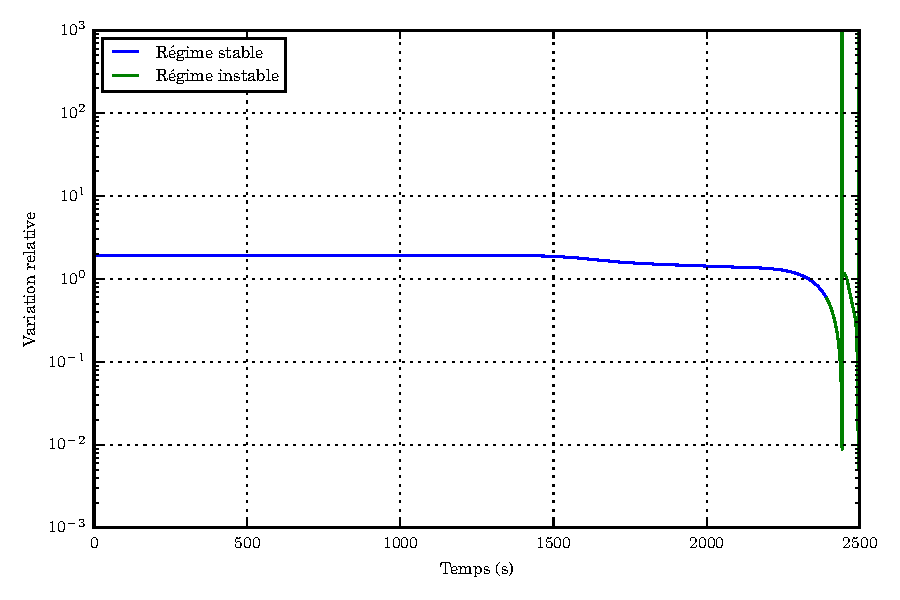
\includegraphics[scale=0.7]{df_dS_and_df_dT.pdf}
    \end{center}
\end{frame}
%--------------------------


\subsection{Domaine instable}

\begin{frame}
  \frametitle{Intégration hors du domaine stable}
  \uncover<1->{
    \begin{equation}\begin{aligned}
      S^{t+1}_n  &= S_{n-1}^{t}\left(\frac{\Delta t}{\Delta x^2}\frac{\nu_{n-1}^t}{x_n^2}\right)\\
               &+ S_n^{t}\left(1 - 2\frac{\Delta t}{\Delta x^2}\frac{\nu_n^t}{x_n^2}\right) \\
               &+ S_{n+1}^{t}\left(\frac{\Delta t}{\Delta x^2}\frac{\nu_{n+1}^t}{x_n^2}\right) \\
    \end{aligned}\end{equation}  
  }
  \uncover<2->{
    Instable ssi
    \begin{equation}
      \bigg(\underbrace{\frac{\Delta x^2}{\Delta t} \bigg.}_\mathrm{vit. num.}\bigg)^{-1} \times
      \underbrace{\bigg.\frac{\nu}{x^2}}_\mathrm{vit. diff.} > 0.5
    \end{equation}
  }
  
\end{frame}

\section{Résultats}
\subsection{Régime stable}

\begin{frame}
  \begin{figure}
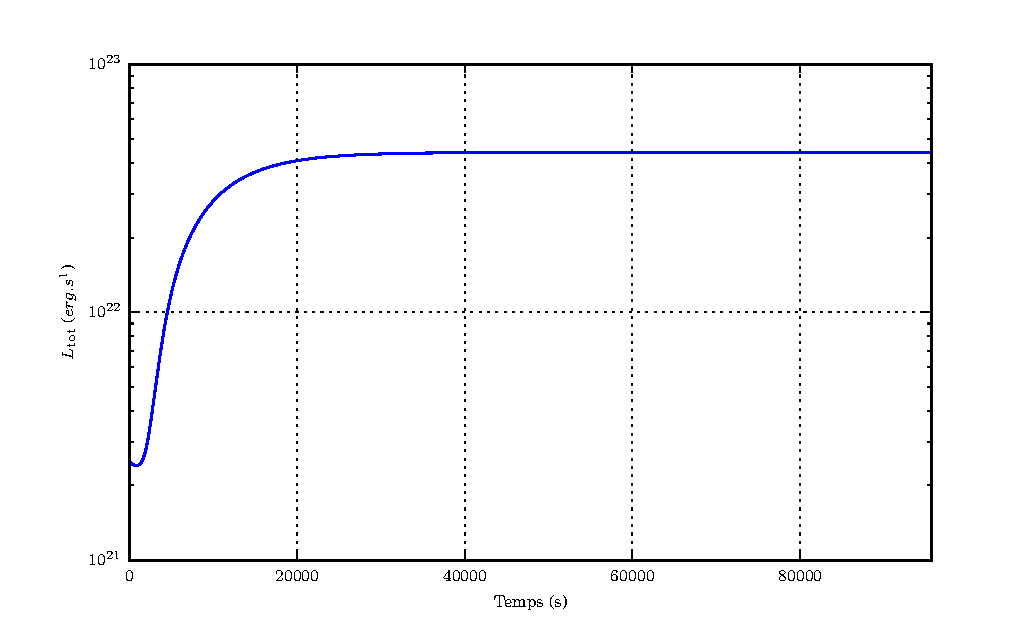
\includegraphics[width=\columnwidth]{figures/Ltot_fonction_t_stable.pdf}
    \caption{Évolution température en fonction du temps, $\dot{M}_0 = 10^{-3}\dot{M_c}$.}
  \end{figure}
\end{frame}

\subsection{Régime instable}

\begin{frame}
  \begin{figure}
    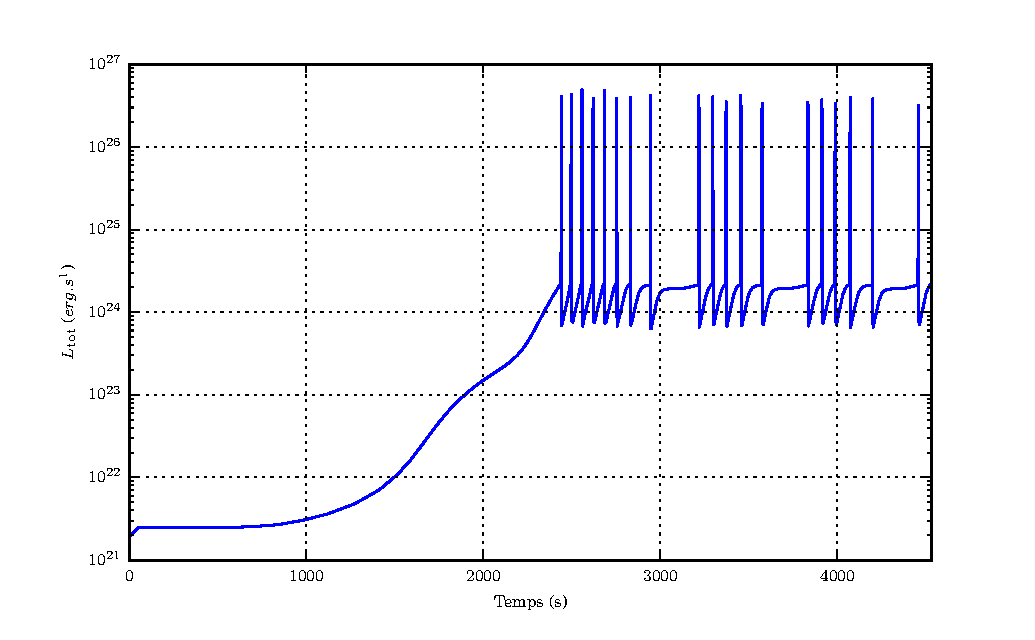
\includegraphics[width=.9\columnwidth]{figures/Ltot_fonction_t.pdf}
    \caption{Évolution température en fonction du temps, $\dot{M}_{t=0}$ variable.}
  \end{figure}  
\end{frame}
\end{document}

\grid
